\documentclass[a4paper,11pt]{report}
\usepackage[utf8]{inputenc}
\usepackage[T1]{fontenc}
\usepackage[francais]{babel}
\usepackage{graphicx}
\usepackage{geometry}
\usepackage{listings}




\title{Machines Virtuelles}
\author{Edgar RODRÍGUEZ}


\begin{document}
\maketitle

\subsection{Machines virtuelles}
La virtualisation consiste à faire fonctionner sur un seul ordinateur plusieurs
systèmes d'exploitation comme s'ils fonctionnaient sur des ordinateurs distincts.
Une machine virtuelle est un conteneur fermement isolé capable d’exécuter ses
propres système d’exploitation et applications, à l’instar d’un ordinateur physique.
Elle se comporte exactement comme un ordinateur physique, elle est totalement indépendante du matériel physique sous-jacent. Par exemple, on peut configurer une machine virtuelle avec des composants virtuels (comme un processeur, une carte réseau) qui diffèrent des composants physiques présents dans la machine hôte ce qui donne de nombreux avantages.
 On
appelle serveur privé virtuel (Virtual Private Server ou VPS) ou encore
environnement virtuel (Virtual Environment ou VE) ces ordinateurs virtuels.
Indépendance vis-à-vis matériel 


Les machines virtuelles constituent un module fondamental d’une solution bien plus conséquente : l'infrastructure virtuelle. Tandis qu’une machine virtuelle reproduit les ressources matérielles d’un ordinateur complet, une infrastructure virtuelle représente l’interconnexion des ressources matérielles d’une infrastructure informatique complète, en y incluant ordinateurs, périphériques réseau et ressources de stockage partagées. Des organisations de toutes tailles utilisent des solutions VMware pour configurer un serveur virtuel et des infrastructures de postes de travail virtuels visant à améliorer la disponibilité, la sécurité et la gérabilité des applications critiques pour l’entreprise. 

\subsection{OpenVZ}
OpenVZ est une technologie base de Virtuozzo développé par SWsoft sous licence conformément aux termes de la GNU GPL version 2, de virtualisation au niveau du système d'exploitation Linux (niveau noyau) ce qui permet une meilleure gestion des ressources et des performances accrues par rapport à une virtualisation système. OpenVZ permet à un serveur physique d'exécuter plusieurs instances isolées du système d'exploitation, appelés environnements virtuels (VE).
Par rapport aux machines virtuelles telles que VMware, VirtualBox et les technologies de virtualisation comme Xen, OpenVZ offre moins de flexibilité dans le choix du système d'exploitation: il faut que le système hôte et le système invité soit de base Linux (bien que les distributions de GNU / Linux peut être différent dans différentes VE). Cependant, la virtualisation OpenVZ niveau de fonctionnement du système offre de meilleures performances, l'évolutivité, la densité, la gestion dynamique des ressources, et la facilité d'administration que les solutions de rechange.
OpenVZ est une base de Virtuozzo est un logiciel commercial développé par SWsoft, Inc OpenVZ est un produit de logiciel libre sous licence conformément aux termes de la GNU GPL version 2. 
\begin{itemize}
  \item 
\end{itemize}

\subsection{KVM}
KVM permet la virtualisation de tout système d'exploitation sur des processeurs d'architectures x86 disposant des technologies Intel VT ou AMD-V.
KVM a lieu en tant que module du noyau Linux, ce module exporte un périphérique appelé /dev/ kvm permet un mode d'hôtes en plus d'autres modes d'utilisation traditionnels qui prend en charge le noyau. Dans un arbre traditionnel /dev dispositifs sont communs à tous les processus dans l'espace utilisateur, mais dans /dev/ kvm à chaque processus qui est lancé est associé à un mappage de périphérique différent.
Cela garantit une isolation entre les machines virtuelles. Lorsque le module est installé KVM, le noyau Linux devient un hyperviseur. Un hyperviseur peut exploiter tous les avantages d'un noyau Linux standard.
Utilisation de systèmes d'exploitation invités KVM peut lancer dans l'espace utilisateur. Chaque système d'exploitation invité est un processus distinct au sein du système d'exploitation hôte. Ci-dessus mais en dessous des systèmes d'exploitation invités il ya une couche très mince (QEMU dans ce cas), qui est l'interface pour la gestion, le contrôle et la configuration des machines virtuelles.

\subsection{Proxmox VE}

Proxmox Virtual Environment est un logiciel libre de virtualisation, plus précisément un hyperviseur de machine virtuelle. Il est développé et maintenu par Proxmox Server Solutions GmbH.
C'est une solution de virtualisation "bare metal" c'est-à-dire qu'on commence à partir d'un serveur vide et qu'il n'y a donc aucune besoin d'installer un système d'exploitation auparavant.
Proxmox VE installe les outils complets du système d'exploitation et de gestion rapidement.
Le logiciel inclut:
\begin{itemize}
  \item Système d'exploitation complet (Debian Lenny 64 bits)
  \item Interface web pour l'administration et la surveillance (création de VM de différents OS, démarrage et arrêt sauvegarde et restore et Migration).
  \item Noyau Proxmox VE avec support d'OpenVZ et de KVM.
  \item Outils de sauvegarde et de restauration.
  \item Partitionnement de disque dur avec LVM2.
  \item Une plateforme de virtualisation (et de 
supervision de VM) pour les opérations de base: Créer, détruire, paramétrer, lancer, arrêter, sauvegarder et déplacer.
  \item Fonctions de clustering qui permet la migration à chaud des machines virtuelles d'un serveur physique à un autre (en utilisant un stockage partagé).
Un «cluster» Proxmox est un regroupement de plusieurs serveurs physiques composé de 1 ou plusieurs noeuds.
\end{itemize}

Système requis:
\begin{itemize}
   \item CPU 64 bits (Intel EM64T ou AMD64)
   \item 2 GB de RAM ou plus (pas limité grâce au noyau 64 bits)
   \item CPU 64 bits (Intel EM64T ou AMD64), microprocesseur multi cœur recommandé
Carte-mère et BIOS compatible Intel VT/AMD-V (pour le support de la virtualisation par KVM)
\end{itemize}

\subsubsection{Installation Proxmox VE}\\
La configuration la plus important au commence de l'installation.\\
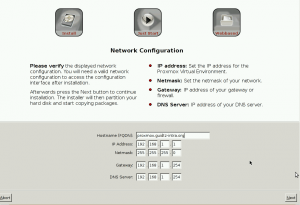
\includegraphics[width=0.5\textwidth]{img/installation.png}\\
\caption{Configuration du réseau }


Proxmox VE met à disposition une interface d’adminsitration web, pour s’y connecter, entrez l’adresse IP de la machine ou une URL y pointant. Une fois loggué on arrive sur la fenêtre suivante:\\
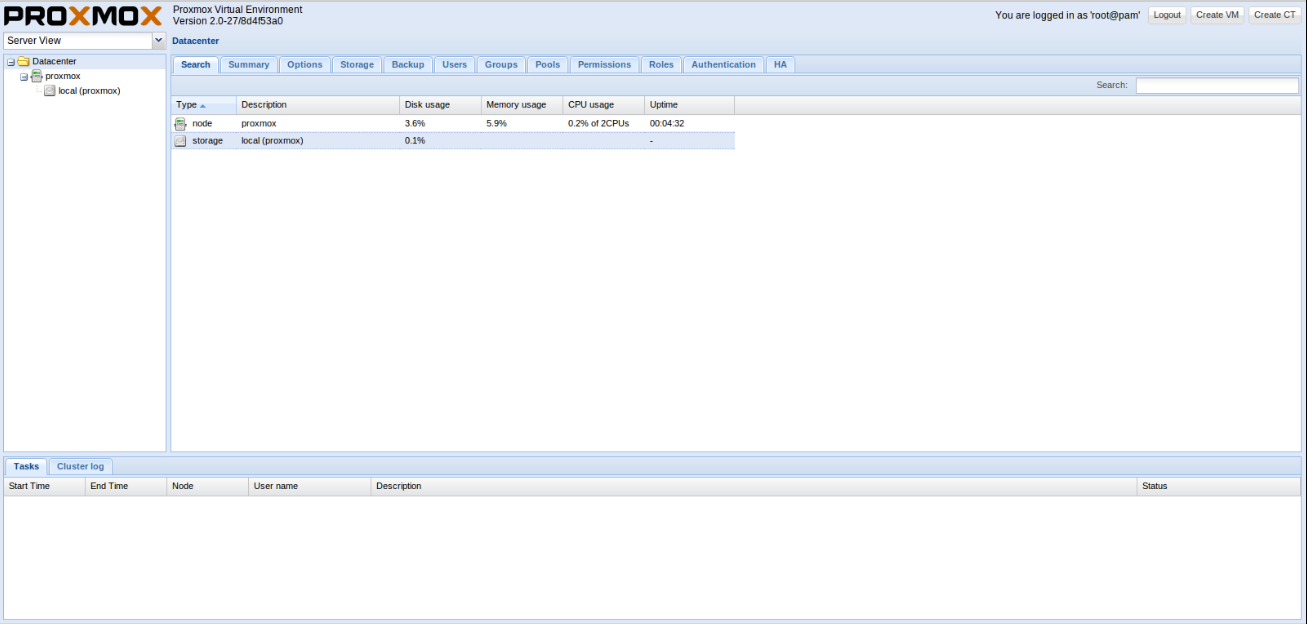
\includegraphics[width=0.5\textwidth]{img/premiere.png}\\
\caption{Fenêtre aprés de se logguer. }\\

\\
Pour créer une machine virtuelle on lance l'option "Create VM" et on met tous les paramètres pour la nouvelle machine (système d'exploitation, disque dur, mémoire, processeur interface réseau).\\
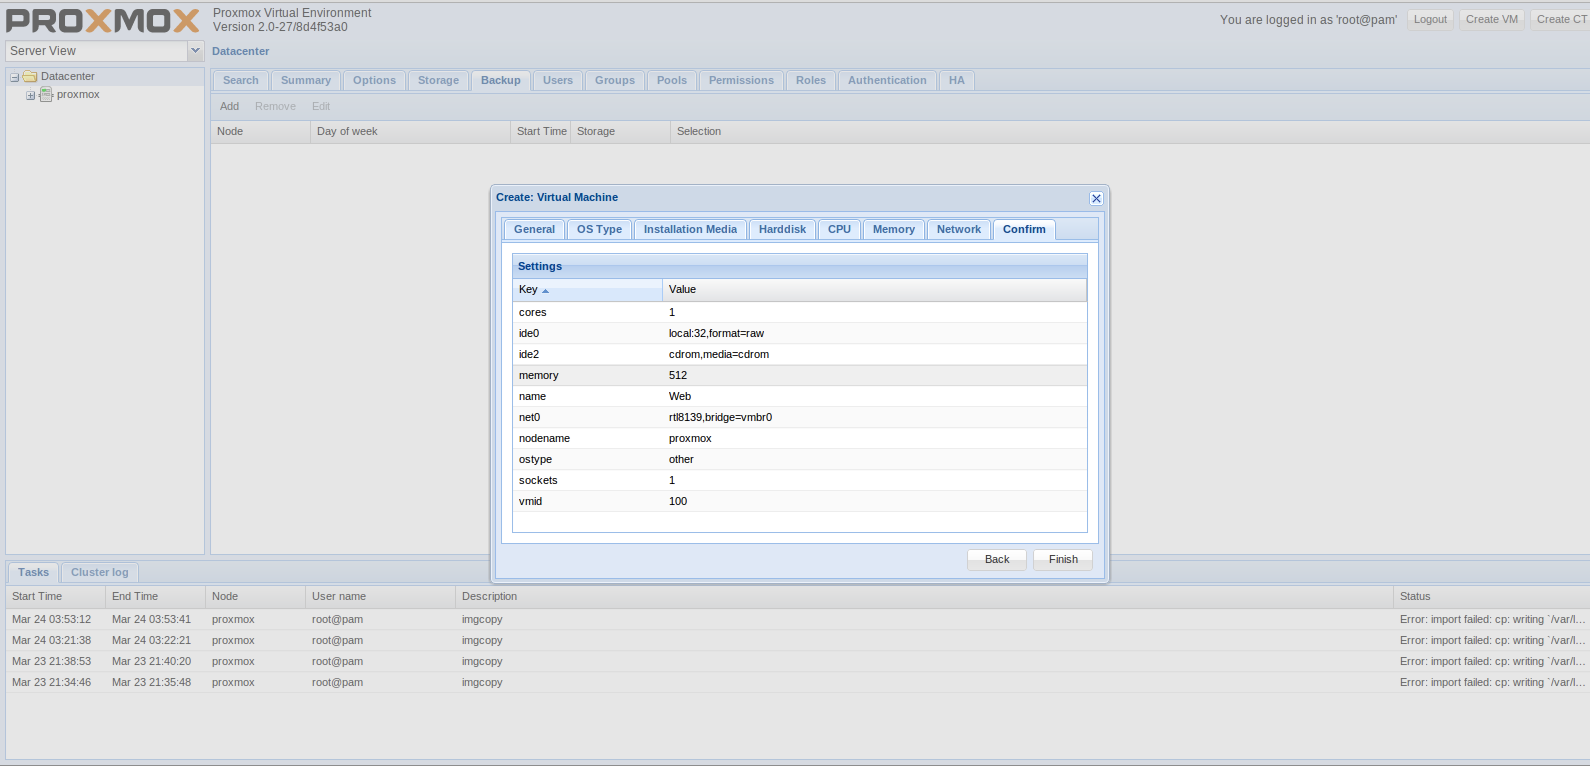
\includegraphics[width=0.5\textwidth]{img/creation-VM.png}\\
\caption{Un résumé d'une configuration d'une VM. }\\




\subsubsection{Sauvegarde et restauration d'une VM}

Vzdump permet de sauvegarder et de restaurer des VM, il est un utilitaire pour prendre des instantanés (snapshots) compatibles de fonctionnement OpenVZ conteneurs (et des machines virtuelles KVM, si nous utilisons VE Proxmox). C'est un script PERL basé sur les commandes tar, gzip, rsync, lvm et vzctl. Il crée une archive tar de la zone privée du conteneur, qui comprend également les fichiers de configuration CT. Il y a plusieurs façons d'assurer la cohérence: Arrêter le CT lors de la sauvegarde (temps d'arrêt très long), utiliser rsync et suspend / commencer (temps d'arrêt minimal) et l'utilisation de LVM2 (aucun temps d'arrêt). Vzdump stocke la sauvegarde sur le disque dans un fichier unique, ce fichier devrait être stocké à une sauvegarde sur bande pour l'archivage.


\subsubsection{Sauvegarder une machine virtuelle arrêtée}


Si on a la possibilité d'arrêter le serveur, cette mesure est la meilleure. Le VE est arrêté, sauvegardée, puis redémarré. Cette opération dure quelques minutes et on ne prend aucun risque par rapport à l'intégrité de la sauvegarde.

Pour sauvegarder la machine virtuelle numéro 105, on utilise la commande:
\begin{lstlisting}
# vzdump --stop --compress --tmpdir /var/lib/vz/vztmp/ 105
\end{lstlisting}
\begin{itemize} 
   \item --stop stop/start VM si est allumée
   \item --compress comprime le fichier dump (gzip)
   \item --tmpdir stocke les fichiers temporaires dans le dossier DIR.  --suspend and --stop
   \item répertoire où sera stockée la sauvegarde
   \item id de la machine virtuelle
\end{itemize}
Le fichier de sauvegarde compressé vzdump-105.tgz est créé dans le répertoire /var/lib/vz/vzdump par défaut.

\subsubsection{Sauvegarder une machine virtuelle à chaud}

Si la VM doit rester allumé, cas d'un serveur de production, vzdump peut procéder à faire une copie à chaud dont deux solutions sont disponibles.


\subsubsection{Sauvegarder à chaud avec une interruption de service}

vzdump procéde en 3 étapes :
\begin{itemize} 
   \item Il duplique la VM à chaud, celui restant actif.
   \item La VM est suspendu et re-synchronisé avec la copie.
   \item Il reprend la VM suspendu.
\end{itemize}
L'interruption de service dure quelques secondes.

\begin{lstlisting}
# vzdump --suspend --compress --tmpdir /var/lib/vz/vztmp/ 105
\end{lstlisting}
\begin{itemize} 
   \item --suspend suspendre/reprendre la VM lors de l'exécution
\end{itemize}
   

\subsubsection{Sauvegarder à chaud sans interruption de service}

Ce type de sauvegarde nécessite l'utilisation de LVM, vzdump fait un snapshot LVM à chaud sans aucune interruption de service.
Pour cette opération, il doit rester suffisamment d'espace libre sur le volume group pour la création du snapshot.

\begin{lstlisting}
# vzdump --snapshot --compress --tmpdir /var/lib/vz/vztmp/  101
\end{lstlisting}
\begin{itemize} 
   \item --suspend utilise LVM snapshot lors de l'exécution
\end{itemize}

\subsubsection{Restaurer une VM clonée}

On utilise une des sauvegardes crées avant.
\begin{lstlisting}
# vzrestore /var/lib/vz/dump/vzdump-105.tgz 103
\end{lstlisting}

On doit reconfigurer les paramètres du réseau au clone car pour l'instant, la machine 103 à la même configuration que la machine 105. 
\begin{lstlisting}
# vzctl set 103 --ipdel 192.168.0.105 --ipadd 192.168.0.103  --hostname clone103 --save
\end{lstlisting}
\end{document} 